\documentclass[../Cours.tex]{subfiles}

\usepackage{xstring}
\usepackage{xfp}

\begin{document}
\clearpage
\thispagestyle{empty}

\newcommand{\bionic}[2][0.5]{%
% split on first space
\StrCut{#2}{ }{\nextword}{\otherwords}%
% count length of first word
\exploregroups%
\StrLen{\nextword}[\currlen]%
% calculate nr. of characters for left part
\edef\halflen{\fpeval{ceil(\currlen*#1)}}%
% print left part in bold
\bfseries\StrLeft{\nextword}{\halflen}%
% print right part and add space back
\normalfont\StrGobbleLeft{\nextword}{\halflen}\space%
\noexploregroups%
% call function recursively if there are other words
\IfStrEq{\otherwords}{}{}{%
\bionic[#1]{\otherwords}%
}}

\setcounter{DS}{1}

\newcommand{\nomPrenom}{%
    Nom : \rule{2cm}{1pt}  \hfill Prénom : \rule{2cm}{1pt} \hfill Classe : \rule{2cm}{1pt}
}

\newcommand{\caseReponse}[1]{%
    \vspace{-1.2em}%
    \begin{center}
    \begin{tikzpicture}
        \draw (0,0) rectangle (\textwidth,#1);
    \end{tikzpicture}
    \end{center}
}

\color{black}
\nomPrenom
\titreDS

\begin{questions}
    \EXERCICETITRE{4}{Multiplication ou division ?}
    \textit{Dans cet exercice, on posera chaque calcul et on fera une phrase réponse.}
    \question Un apiculteur vend le miel qu'il produit \qty{15}{\EURO} pour \qty{1}{\kilo\gram}.\\ Combien va-t-on payer si on achète \qty{7}{\kilo\gram} ? \caseReponse{2.2}
    \question \qty{3}{\litre} de peinture coûte \qty{75,30}{\EURO}. Combien coûte \qty{1}{\litre} de peinture ? \caseReponse{2.2}
    \question On veut ranger 153 livres sur des étagères. Chaque étagère peut contenir 25 livres. De combien d'étagères aura-t-on besoin ? \caseReponse{2.2}
    \question Combien y a-t-il de secondes dans une journée ? \caseReponse{2.2}

    \EXERCICETITRE{6}{Symétrie axiale}
    \question Construire le symétrie de la figure $(\mathcal{F})$ par rapport à la droite $(d)$.
    \begin{center}
    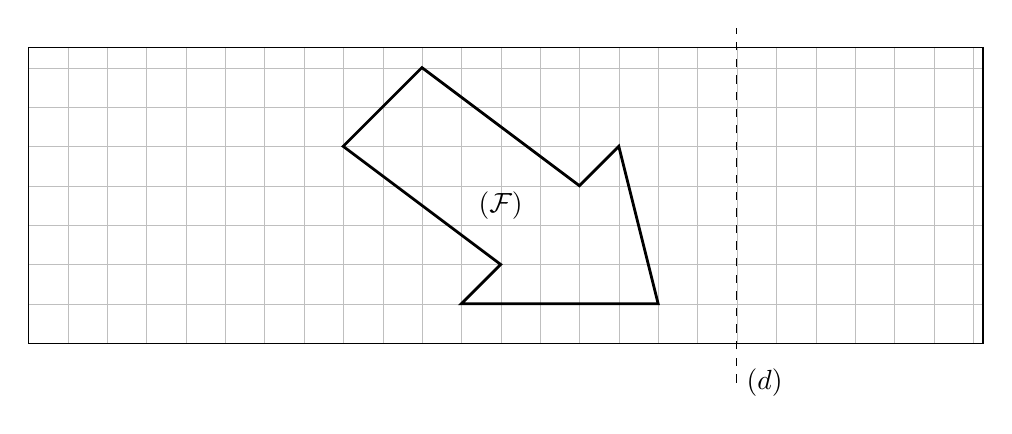
\begin{tikzpicture}[scale=0.5]
        \draw[line width=0.01mm,gray!50!white] (-8,-1) grid +({2*\textwidth},7.5);
        \draw (-8,-1) rectangle +({2*\textwidth},7.5);
        \draw[dashed] (10,-2) -- (10,7);
        \node[right] at (10,-2) {$(d)$};
        \node at (4,2.5) {$(\mathcal{F})$};
        \draw[line width=1pt] (6,3) -- (7,4) -- (8,0) -- (3,0) -- (4,1) -- (0,4) -- (2,6) -- cycle;
    \end{tikzpicture}
    \end{center}

    \clearpage 
    \question Construire le symétrique de la figure $(\mathcal{G})$ par rapport à la droite $(e)$.
    \begin{center}
    \begin{tikzpicture}[scale=0.5]
        \draw (-8,-5) rectangle +({2*\textwidth},12);
        \draw[dashed] (9,-3) -- (11.33,7);
        \node[right] at (9,-3) {$(e)$};
        \node at (4,2.5) {$(\mathcal{G})$};
        \draw[line width=1pt] (6,3) -- (7,4) -- (8,0) -- (3,0) -- (4,1) -- (0,4) -- (2,6) -- cycle;
    \end{tikzpicture}
    \end{center}

    \EXERCICETITRE{5}{Conversion d'unités}
    Voici une liste d'objets avec leur longueur :
    \begin{itemize}
        \item Une règle : \qty{3}{\deci\metre}
        \item Un lingot d'or : \qty{31,5}{\milli\metre}
        \item Un pouce : \qty{2,54}{\centi\metre}
        \item Une télécommande : \qty{0,2}{\metre}
    \end{itemize}

    \question Convertir ces 4 longueurs en \unit{\milli\metre} \caseReponse{3}
    \question Ranger ces quatre objets dans l'ordre croissant \caseReponse{2}

    \clearpage
    \EXERCICETITRE{5}{Aller plus loin : la conjecture de Syracuse}

    On part d'un nombre donné. S'il est pair, on le divise par 2. S'il est impair, on le multiplie par 3 et on ajoute 1. Puis on recommence jusqu'à ce qu'on arrive au nombre 1.\\

    Par exemple, si on prend 5, comme 5 est impair, le suivant sera $5 \times 3 + 1 = 16$. Puis comme 16 est pair, le suivant sera $16 \div 2 = 8$. Comme 8 est pair, le suivant sera $8 \div 2 = 4$. Puis 4 est pair, donc le suivant est $4 \div 2 = 2$. Enfin, 2 est pair, donc le suivant est $2 \div 2 = 1$. On a atteint le nombre 1, on s'arrête là.

    \question Faire cette chaîne de calcul en partant du nombre 7 \caseReponse{3}
    \question Faire cette chaîne de calcul en partant du nombre 15 \caseReponse{3}
    
    
\end{questions}
\end{document}